\documentclass[
	12pt, % Default font size, values between 10pt-12pt are allowed
	%letterpaper, % Uncomment for US letter paper size
	%spanish, % Uncomment for Spanish
]{fphw}

\usepackage[utf8]{inputenc} 
\usepackage[T1]{fontenc}
\usepackage{mathpazo}\usepackage{graphicx} 
\usepackage{booktabs} 
\usepackage{listings} 
\usepackage{enumerate} 

\title{Assignment \#1} %
\author{Anita Mezzetti} 
\institute{École polytechnique fédérale de Lausanne} 
\class{Global Business Environment} 
\professor{Luisa Lambertini} 

%--------------------------------------------------------------------
\begin{document}

\maketitle 
\chapter{Part I}
\section*{Question 1}

B \\
\par The GDP is the value of all final values and services produced within a country. In an open economy, we have to subtract the imports from total domestic spending. To prove it we have the national income identity: $Y=C+I+G+EX-IM$, where Y is the GDP.

%----------------------------------------------------------------------------------------

\section*{Question 2}
A \\
\par The GDP has a geographical definition: to understand what we have to include in the GDP we have to check if that good/service is produced within the borders of a nation. \\If we were talking about GNP we would consider the production of country's factors. \\
Moreover we include only the final goods and services, excluding illegally goods.
%----------------------------------------------------------------------------------------

\section*{Question 3}
C \\
\par It's important to notice that the sale of a used textbook doesn't concern the production, because it was already been sold in the past. However it could generate an income. For example, consider that I can be a librarian. I sell the used textbook at a higher price than the price I had bought it. In this case I have an income. 

%----------------------------------------------------------------------------------------

\section*{Question 4}
B \\ 
\par Investments represents the part of value used by firms to produce future output, so to increase the nation's stock of capital. In these investments we include also the purchase of inventories, because carrying inventories is a way to transfer worth from current use to future use. \\
The households' inventories are considered in the consumption.  \\

\newpage
%-----------------------------
\chapter{Part II}
\section*{Question 1}
\begin{figure}[h]
\centering 
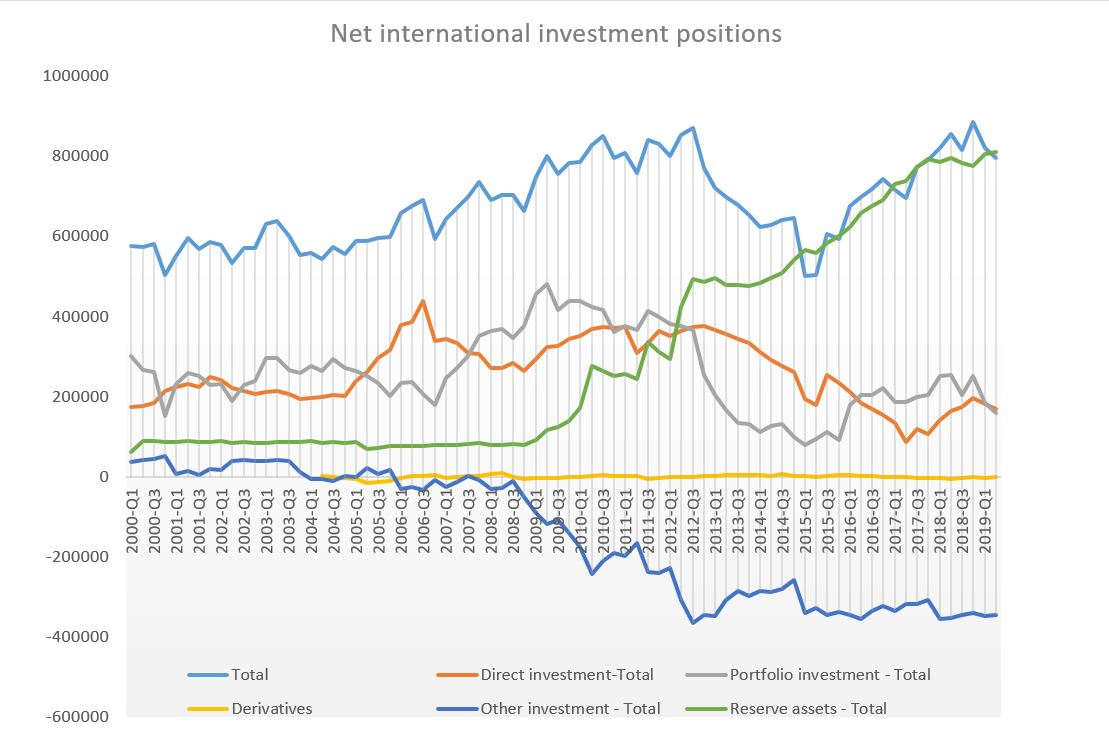
\includegraphics[scale=0.7]{ass1es2pt1.JPG} 
\caption{Part II, Question 1} 
\end{figure}


\section*{Question 2}
This curve illustrates that total NIIP increased from 2007Q3 to 2012Q3 (in this period the Financial crisis and the European dept crisis took place). This growth was irregular, with some ups and downs. \\Then total NIIP rapidly went down, still 2015Q3. In this period reserve assets were rising, but its contribute was not enough: other components were falling. \\
After 2015Q3 total NIIP started again to go up.

\section*{Question 3}
From 2000Q1 to 2007Q3 total NIIP didn't have significant peaks or drops. It's difficult to identify the components which caused the behaviour of the curve.
From 2007Q3 total NIIP increased mainly thanks to the reserve assets curve. \\
Even if the reserve asset was rising, there was a decline between 2012Q3 and 2015Q3. It was caused by all the other components, in particular by the portfolio investments and direct investments. \\
Reserve assets helped total NIIP to grow moderately after 2015Q3. 

\section*{Question 4}
\begin{figure}[h]
\centering 
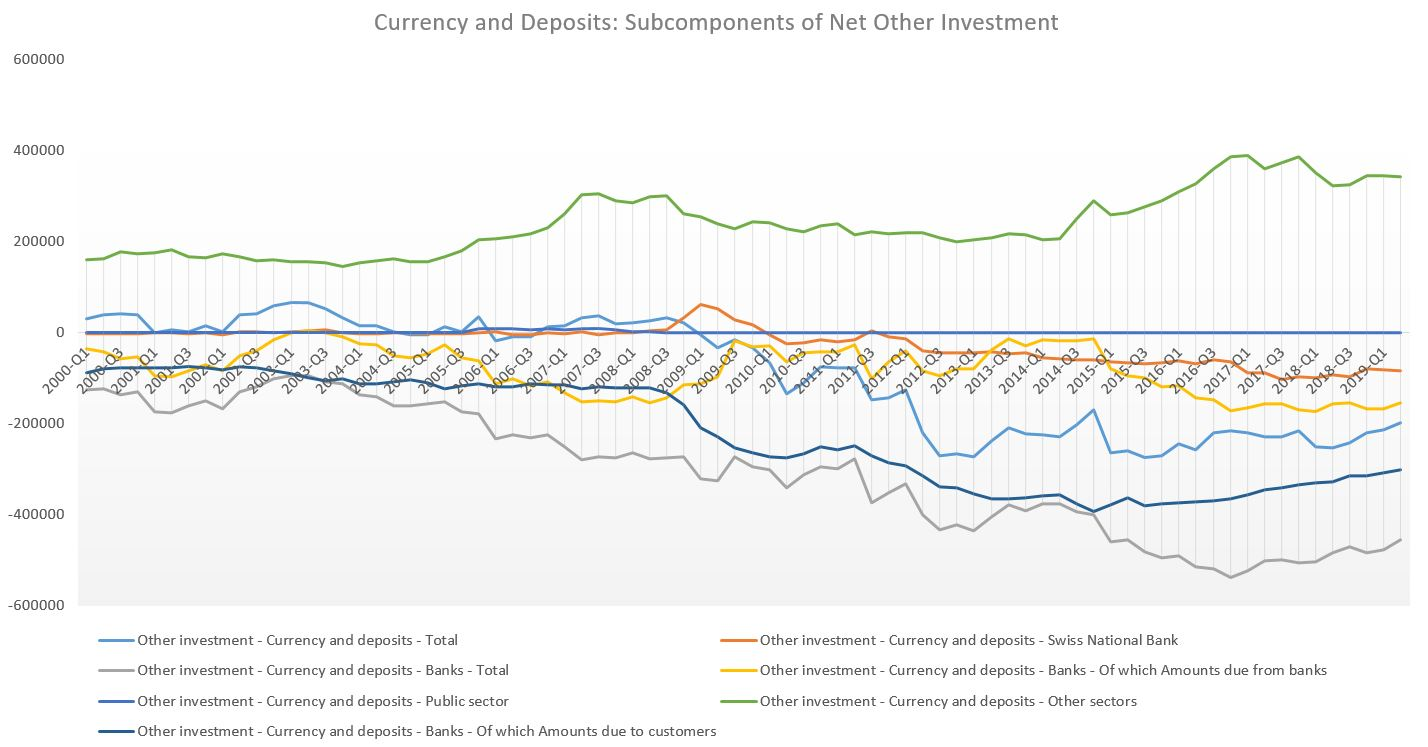
\includegraphics[scale=0.7]{ass1es3pt2.JPG} 
\caption{Part II, Question 4} 
\end{figure}
Other Investment NIIP has gone down since the end of 2007. This means that foreign customers investments increased. \\
We know that the global financial crisis started in 2008. So this graph shows that in this period many nonresidents opened accounts In Switzerland and brought their money here. This happened because this country was seen as a safe and untouchable place. Economically, Switzerland focused on maintaining a stable environment to attract foreign investors.

\section*{Question 5}
The Euro crises affected the Swiss economy: the Swiss franc was rapidly appreciating against the Euro. The economic uncertainty caused by the European debt crisis was the main cause of the strength of the Swiss franc. So the Swiss National Bank increase its quantities of Euro to prevent an excessive appreciation of the local currency. \\
The export industry was particularly affected by the strong value of the franc. To understand why Switzerland wanted to limit the value of franc, we should consider that Switzerland traditionally had a strong export sector; which regularly leads to increase the demand for Swiss francs worldwide to pay for Swiss export products. \\
Financial investors will continue to be attracted as long as the economic prospects for the Eurozone do not stabilise considerably, but the strong Swiss franc risks to reduced Swiss ability to compete in terms of price.





\end{document}